\documentclass{tufte-handout}

%\geometry{showframe}% for debugging purposes -- displays the margins

\usepackage{amsmath, listings}

% Set up the images/graphics package
\usepackage{graphicx}
\setkeys{Gin}{width=\linewidth,totalheight=\textheight,keepaspectratio}
\graphicspath{{graphics/}}

\title{The Zernike Polynomials}
\author{Joshua Cook}
\date{10 December 2014}  % if the \date{} command is left out, the current date will be used

% The following package makes prettier tables.  We're all about the bling!
\usepackage{booktabs}

% The units package provides nice, non-stacked fractions and better spacing
% for units.
\usepackage{units}

% The fancyvrb package lets us customize the formatting of verbatim
% environments.  We use a slightly smaller font.
\usepackage{fancyvrb}
\fvset{fontsize=\normalsize}

% Small sections of multiple columns
\usepackage{multicol}

% Provides paragraphs of dummy text
\usepackage{lipsum}

% These commands are used to pretty-print LaTeX commands
\newcommand{\doccmd}[1]{\texttt{\textbackslash#1}}% command name -- adds backslash automatically
\newcommand{\docopt}[1]{\ensuremath{\langle}\textrm{\textit{#1}}\ensuremath{\rangle}}% optional command argument
\newcommand{\docarg}[1]{\textrm{\textit{#1}}}% (required) command argument
\newenvironment{docspec}{\begin{quote}\noindent}{\end{quote}}% command specification environment
\newcommand{\docenv}[1]{\textsf{#1}}% environment name
\newcommand{\docpkg}[1]{\texttt{#1}}% package name
\newcommand{\doccls}[1]{\texttt{#1}}% document class name
\newcommand{\docclsopt}[1]{\texttt{#1}}% document class option name

\begin{document}

\maketitle% this prints the handout title, author, and date

\begin{abstract}
\noindent A program in Python to generate, evaluate, and visualize Zernike
polynomials, a family of orthogonal polynomials over the unit disk, $D =
\{(\rho, \theta)| 0 \leq \rho \leq 1, 0 \leq \theta \leq 2\pi\}$ and discussions and proofs
of some of their properties.  Zernike
polynomials are used to
describe aberrations in a lens (e.g., the cornea).
\end{abstract}

%\printclassoptions


\section{Description}\label{sec:description}
\newthought{Even and odd Zernike Polynomials} are defined
respectively as

\begin{equation}
Z_n^m(\rho,\theta)=R_m^n(\rho)\cos(m\theta)\ \ \ \ \text{and}\ \ \ \
Z_n^{-m}(\rho,\theta)=R_m^n(\rho)\sin(m\theta)
\end{equation}

where $n,m\in\mathbb{Z}, n\geq m\geq 0$, $\theta$ is the \textit{azimuthal angle}, $\rho$ the
radial distance, and $R^m_n(\rho)$, the radial polynomials given by

\begin{equation}
R^m_n(\rho) = \sum_{k=0}^{\tfrac{n-m}{2}} \frac{(-1)^k\,(n-k)!}{k!\left
(\tfrac{n+m}{2}-k \right )! \left (\tfrac{n-m}{2}-k \right)!} \;\rho^{n-2\,k}
\end{equation}

\paragraph{} Rewriting the ratios of factorials in the radial part as products of Binomial
coefficient shows that the coefficients are integer numbers:

\begin{equation}
\label{binomial_relation}
R_n^m(\rho)=\sum_{k=0}^{\tfrac{n-m}{2}}(-1)^k \binom{n-k}{k}
\binom{n-2k}{\tfrac{n-m}{2}-k} \rho^{n-2k}
\end{equation}

They satisfy $|Z_n^m(\rho,\theta)|\leq 1|$ for all $\rho\in(0,1)$ and all
$\theta$.

\section{Properties of the Zernike Polynomials}\label{sec:recursive}
\subsection{Generating the Polynomials}
\newthought{Toward a Recursive Method}, we can find a recursive formula to compute Zernike radial
polynomials\cite{honarvar2013recursive}.  The following recurrence relationship has been previously proposed\cite{kintner1976mathematical}

\begin{equation}
R_n^m(\rho)=\frac{1}{K_1}\Big[(K_2\rho^2+K_3)R_{n\ 2}^m (\rho)+K_4R_{n\
4}^m(\rho)\Big]
\end{equation}

for

$$n=m+4,m+6, \dots$$

where the coefficients are given by\cite{janssen2007computing}

\begin{align*}
K_1&=\frac{(n+m)(n-m)(n-2)}{2}\\
K_2&=2n(n-1)(n-2)\\
K_3&=-m^2(n-1)-n(n-1)(n-2)\\
K_4&=-\frac{n(n+m-2)(n-m-2)}{2}
\end{align*}

To initialize the method we specify cases in which $n=m$ and $n-m=2$:\cite{chong2003comparative}

\begin{equation}
R_m^m(\rho)=\rho^m
\end{equation}
\begin{equation}
R_{m+2}^m(\rho)=(m+2)\rho^{m+2}-(m+1)r^m
\end{equation}

Taking a three-term recurrence relation previously derived\cite{prata1989algorithm}

\begin{equation}
R_n^m(\rho)=\rho L_1R_{n-1}^{|m-1|}(\rho)+L_2R_{n-2}^m(\rho)
\end{equation}

where the coefficients $L_1$ and $L_2$ are

\begin{align*}
L_1&=\frac{2n}{m+n}\\
L_2&=\frac{m-n}{m+n}
\end{align*}

We then start with $R_0^0=1$ and can generate all the polynomials.

\subsection{a Recurrence Relation}\label{sec:relation}

\newthought{Janssen and Dirksen} have shown the following integral representation of radial polynomials\cite{janssen2007computing}

\begin{equation}
R_n^m(\rho)=\frac{1}{2\pi}\int_{k=0}^{2\pi}U_n \rho\cos\theta\cos \theta
\end{equation}

where $U_n$ is the Chebyshev polynomial of the second kind and of degree $n$
that satisfies the following\cite{honarvar2013recursive} recurrence relation for $n\geq 2$

\begin{equation}
U_n(x)=2xU_{n-1}(x)-U_{n-2}(x)
\end{equation}

with $U_0(x)=1$ and $U_1(x)=2x$.

\paragraph{}Clearly, the degree of the radial polynomials is equal to the degree of the
Chebshev polynomials of the second kind.

\paragraph{}Furthermore, the azimuthal order equals the frequency of the cosine function.

\paragraph{}Therefore, simply set $x=\rho\cos\theta$ and multiply by $\cos(m\theta)$ to get

\begin{align*}
U_n(\rho\cos\theta)\cos(m\theta)&=2\rho\cos\theta
U_{n-1}(\rho\cos\theta)\cos(m\theta)-U_{n-2}(\rho\cos\theta)\cos(m\theta)\\
U_n(\rho\cos\theta)\cos(m\theta)&=\rho\Big[\cos(|m-1|\theta)+\cos((m+1)\theta)\Big]U_{n-1}(\rho\cos\theta)cos(m\theta)-U_{n-2}(\rho\cos\theta)\cos(m\theta)\\
\int_0^{2\pi}U_n(\rho\cos\theta)\cos(m\theta)\ d\theta&=\\
\int_0^{2\pi}\bigg(\rho&\Big[\cos(|m-1|\theta)+\cos((m+1)\theta)\Big]U_{n-1}(\rho\cos\theta)cos(m\theta)-U_{n-2}(\rho\cos\theta)\cos(m\theta)\bigg)\ d\theta\\
\end{align*}

\paragraph{}Using the integral representation of radial polynomials, we have the following recurrence relation

\begin{equation}
R_n^m(\rho)=\rho\Big[R_{n-1}^{|m-1|}(\rho)+R_{n-1}^{m+1}(\rho)\Big]-R_{n-2}^m(
\rho)
\end{equation}

or


\begin{equation}
R_n^m(\rho)+R_{n-2}^m(\rho)=\rho\left[R_{n-1}^{\left|m-1\right|}(\rho)+R_{n-1}^
{m+1}(\rho)\right]
\end{equation}

\subsection{Orthogonality}
\newthought{Two functions} $F_1$ and $F_2$ are orthogonal over a unit cirle if:

$$\int_0^1\int_0^{2\pi} F_1F_2\rho d\theta d\rho = 0$$

For axisymmetric functions with no $\theta$ variance, this reduces to

$$2\pi \int_0^1 F_1F_2 \rho d\rho = 0$$

Consider $F_1=\rho^2$ and $F_2=\rho^4$.

$$2\pi\int_0^1 \rho^2 \rho^4\rho  d\rho = \frac{\pi}{4}\neq 0$$

Consider $F_3=2\rho^2-1$ and $F_4=6\rho^4-6\rho^2+1$.

$$2\pi\int_0^1 (2\rho^2-2)(6 \rho^4-6\rho^2+1)\rho  d\rho = 0$$

These are Zernike polynomials.  In fact, the Zernike polynomials are created by
subtracting lower order polynomials to create this orthogonality relationship.

\paragraph{}We seek:

$$\int_0^1\int_0^{2\pi} R_i(\rho)\Theta_i(\theta)R_j(\rho)\Theta_j(\theta)\rho
d\theta d\rho = \delta_j=\left\{
     \begin{array}{lr}
        C_j&  i=j\\
       0 & i\neq j
     \end{array}
   \right.$$

\begin{align*}
\int_0^1R_iR_j\rho d\rho\int_0^{2\pi} \Theta_i\Theta_jd\theta  &= \delta_j\\
\end{align*}

For a $2\pi$-periodic function, we can chose an orthogonal basis (in fact,
orthonormal) in the trigonometric functions $\sin n\theta$ and $\cos n\theta$.
Therefore, our problem is reduced to finding an orthogonal radial basis.

\begin{align*}
\int_0^1R_iR_j\rho d\rho &= \delta_j\\
\end{align*}

\pagebreak

\section{The Program}\label{sec:program}

\newthought{The program consists} of two files, a View file (\Verb|menu.py|) and a Controller file (\Verb|notebook.py|).


\subsection{Controller File}
\paragraph{}\Verb|notebook.py| consists of two classes \Verb|Zernike_Polynomial| and \Verb|Polynomial_Notebook|.  The first is an object representing a specific polynomial, where as the second is an object containing multiple polynomial instances.

\paragraph{Instantiaton of a Notebook}
Each \Verb|Polynomial_Notebook| has several notebook level variables and lists. These include:

\begin{description}
\item[\Verb|self.polynomials|] A list containing polynomials created.
\item[\Verb|self.density|] The density to be used for the plotting of polynomials.
\item[\Verb|self.rho|] A numpy array containing possible radial values.
\item[\Verb|self.theta|] A numpy array containing possible angular values.
\item[\Verb|self.Rho|] A meshgrid object associated with radial values.
\item[\Verb|self.Theta|] A meshgrid object associated with angular values. 
\end{description}

\paragraph{Instantiation of a Polynomial}
Calling \Verb|new_polynomial(m,n)| initializes a new instance of a Zernike polynomial with the passed $m$ and $n$ values.  It does so by calling the following methods from the \Verb|Zernike_Polynomial| class.

\begin{marginfigure}%
  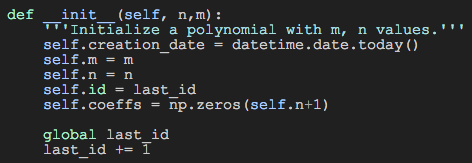
\includegraphics[width=\linewidth]{img/init.png}
  \caption{The polynomial initialization method.}
  \label{fig:init}
\end{marginfigure}

\begin{description}
\item[\Verb|zernike\_Rcoeffs()|] Uses the binomial relationship defined in eq. \ref{binomial_relation} to generate the coefficients of the indicial degree.
\item[\Verb|zernike\_even()|] Generates a mesh-grid, \Verb|Z_even|, representing the multi-variate function $Z_n^m(\rho,\theta)$ on the domain $[0, 1] \times [0, 2\pi]$ using the coefficients generated by \Verb|zernike_Rcoeffs()|.
\item[\Verb|zernike\_odd()|] Generates a mesh-grid, \Verb|Z_odd|, representing the multi-variate function $Z_n^{-m}(\rho,\theta)$ on the domain $[0, 1] \times [0, 2\pi]$ using the coefficients generated by \Verb|zernike_Rcoeffs()|.
\end{description}

\begin{marginfigure}%
  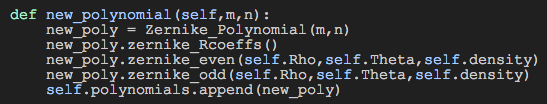
\includegraphics[width=\linewidth]{img/new_poly.png}
  \caption{Method creating a new polynomial instance.}
  \label{fig:init}
\end{marginfigure}

\paragraph{Preparation of Plots}
Plots are generated using the \Verb|matplotlib| commands \Verb|pcolormesh| and \Verb|plot_surface|. The meshgrid objects \Verb|notebook.Rho|, \Verb|notebook.Theta|, \Verb|poly.Z_even|, and \Verb|poly.Z_odd| are used. \Verb|pcolormesh| uses a polar projection. \Verb|plot_surface| uses a cartesian projection in three dimensions requiring the conversion of the meshgrid of cartesian coordinates.


\subsection{View File}

\paragraph{}\Verb|menu.py| imports both classes from \Verb|notebook.py| and adds another \Verb|Menu|.  Instantiating the \Verb|Menu| also instantiates a new \Verb|Polynomial_Notebook|.  

\begin{marginfigure}%
  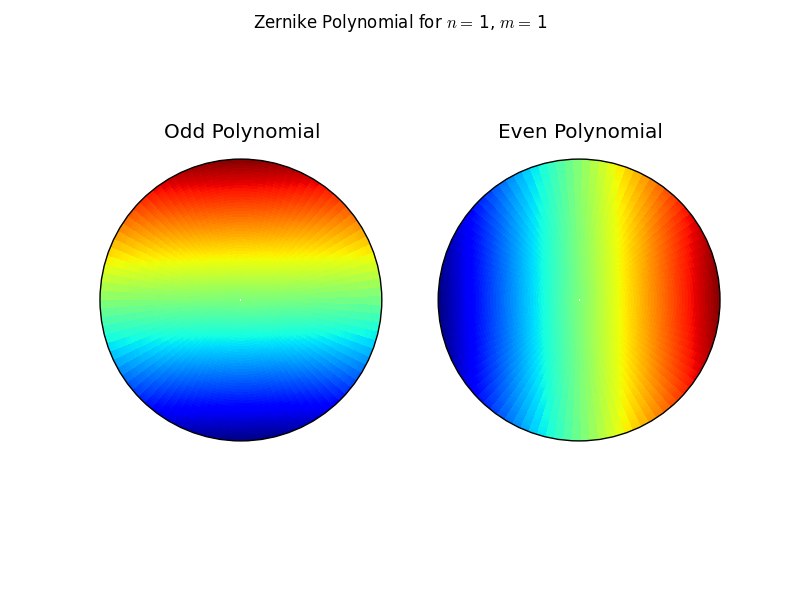
\includegraphics[width=\linewidth]{img/1-1.png}
  \caption{Even and Odd Plots, $n=1$, $m=1$}
\end{marginfigure}

\paragraph{}The methods included as part of the \Verb|Menu| are designed to manipulate this notebook.  Running the menu from the command line provides the user with the following menu:

\begin{verbatim}
Notebook Menu
1. Configure Notebook
2. Add Polynomial
3. Plot Polynomial 
4. Compare 2-D and 3-D plots
5. Quit 
\end{verbatim}

\begin{marginfigure}%
  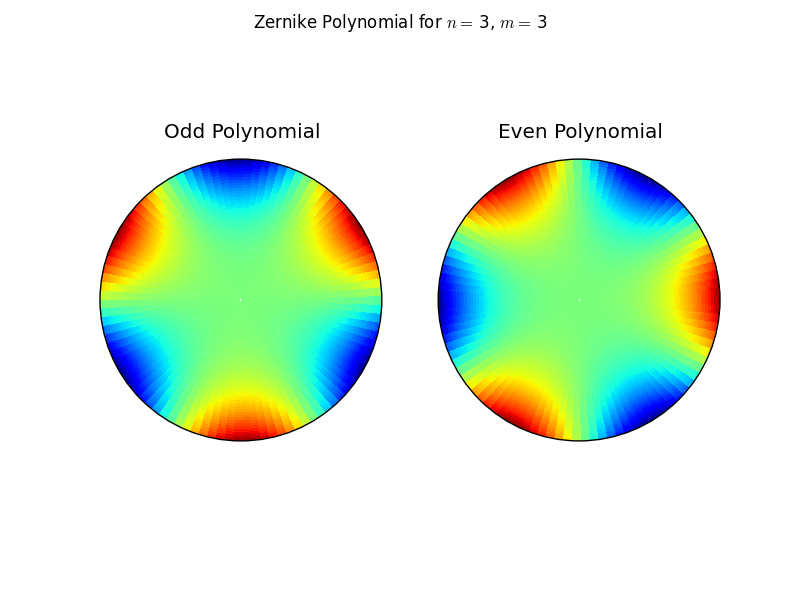
\includegraphics[width=\linewidth]{img/3-3.png}
  \caption{Even and Odd Plots, $n=3$, $m=3$}
\end{marginfigure}

\paragraph{}
\begin{description}
\item[Configure Notebook] Allows the user the change the set density of plots generated.
\item[Add Polynomial] Allows the user to add a polynomial to the notebook.
\item[Plot Polynomial] Generates and displays a plot of the even and odd variants of a particular polynomial.
\item[Compare 2-D and 3-D plots] Generates and displays a plot of an even or odd polynomial in two- and three-dimensions of a particular polynomial.
\item[Quit] Quits the program.
\end{description}

\begin{marginfigure}[-40mm]%
  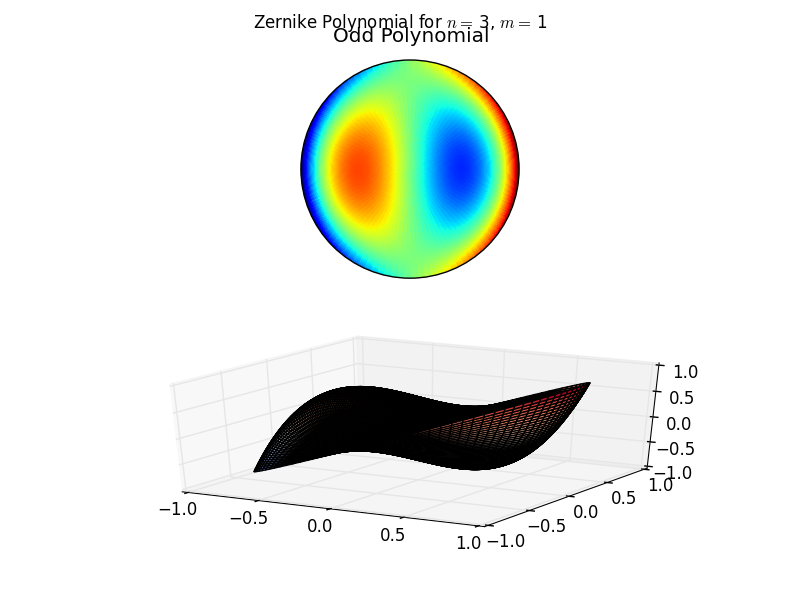
\includegraphics[width=\linewidth]{img/3-1-compare-odd.png}
  \caption{2-D and 3-D plots, Odd polynomial, $n=3$, $n=1$}
\end{marginfigure}

\paragraph{A sample notebook}
After several polynomials have been added, we may see the following polynomials in the notebook after running the \Verb|Show all Polynomials| command:

\begin{marginfigure}[10mm]%
  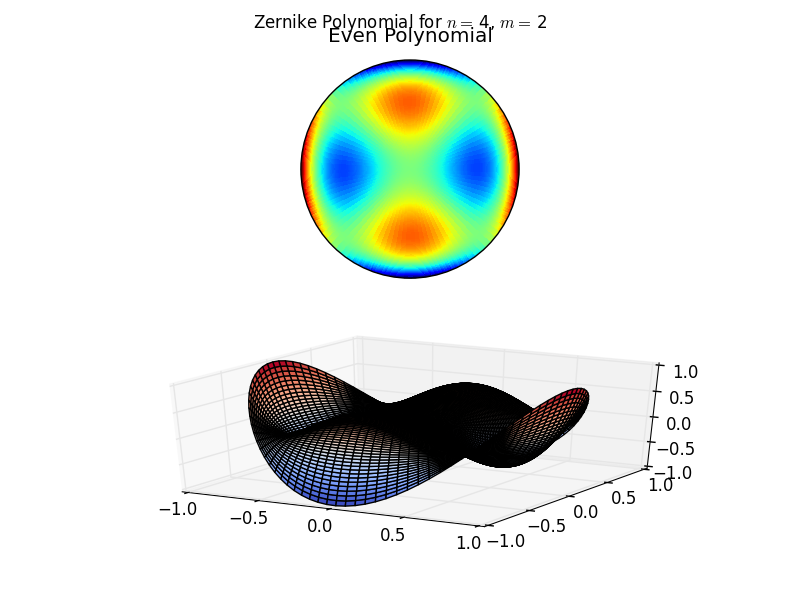
\includegraphics[width=\linewidth]{img/4-2-compare-even.png}
  \caption{2-D and 3-D plots, Even polynomial, $n=4$, $n=2$}
\end{marginfigure}

\begin{verbatim}
1: created: 2014-12-06 n,m: 0,0 coeffs: [ 1.]
2: created: 2014-12-06 n,m: 1,1 coeffs: [ 0.  1.]
3: created: 2014-12-06 n,m: 2,0 coeffs: [-1.  0.  2.]
4: created: 2014-12-06 n,m: 2,2 coeffs: [ 0.  0.  1.]
5: created: 2014-12-06 n,m: 3,1 coeffs: [ 0. -2.  0.  3.]
6: created: 2014-12-06 n,m: 3,3 coeffs: [ 0.  0.  0.  1.]
7: created: 2014-12-06 n,m: 4,0 coeffs: [ 1.  0. -6.  0.  6.]
8: created: 2014-12-06 n,m: 4,2 coeffs: [ 0.  0. -3.  0.  4.]
9: created: 2014-12-06 n,m: 4,4 coeffs: [ 0.  0.  0.  0.  1.]
\end{verbatim}

\pagebreak

\section{The first 15 Zernike Polynomials}


\begin{figure*}[ht]
\centering
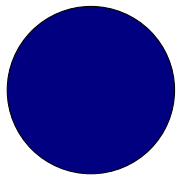
\includegraphics[width=1.25in]{img/orthogonal_polynomials_15_0.png}

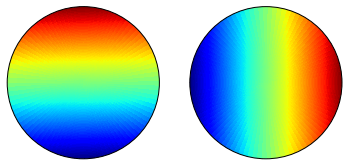
\includegraphics[width=2.5in]{img/orthogonal_polynomials_15_1.png}

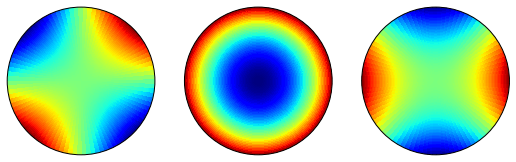
\includegraphics[width=3.75in]{img/orthogonal_polynomials_15_2.png}

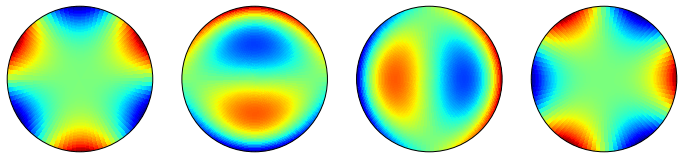
\includegraphics[width=5in]{img/orthogonal_polynomials_15_3.png}

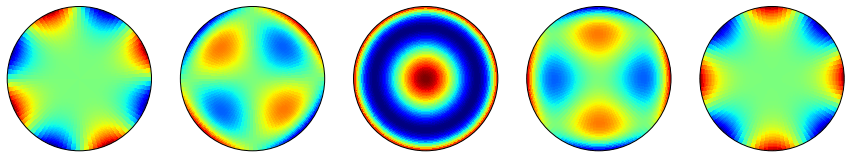
\includegraphics[width=6.25in]{img/orthogonal_polynomials_15_4.png}
\end{figure*}



\end{document}
